
\subsection{Sensitivity to Subgraph Participation: A Comparison with Subgraph Centrality}

Traditional centrality measures---such as degree, closeness, and eigenvector centrality---can sometimes fail to differentiate nodes in highly symmetric or perfectly regular graphs. To address this, \citet{estrada2005subgraph} introduced \emph{subgraph centrality}, a measure that ranks nodes by their participation in all network subgraphs, placing greater weight on smaller motifs (such as triangles and squares). 

To demonstrate the discriminative power of their metric, Estrada and Rodr\'iguez-Vel\'azquez presented two challenging regular graphs: an 8-node regular graph with degree 3, and a 9-node regular graph with degree 6. In both graphs, all nodes have identical degree, identical closeness, and identical eigenvector centrality ($s_i = 1$). However, the nodes differ subtly in their participation in specific subgraphs.

Despite emerging from a fundamentally different theoretical paradigm---one rooted in agonistic competition and structural constraint---distinction centrality ($\beta_i$) perfectly recovers the exact same node rankings as Estrada's subgraph centrality for both of these regular graphs. Figure~\ref{fig:estrada} visualizes the distinction scores for these two networks, and Tables~\ref{tab:estrada1a} and \ref{tab:estrada1b} provide the exact mathematical components.

\begin{figure}[ht!]
    \centering
    \begin{subfigure}[b]{0.45\textwidth}
        \centering
        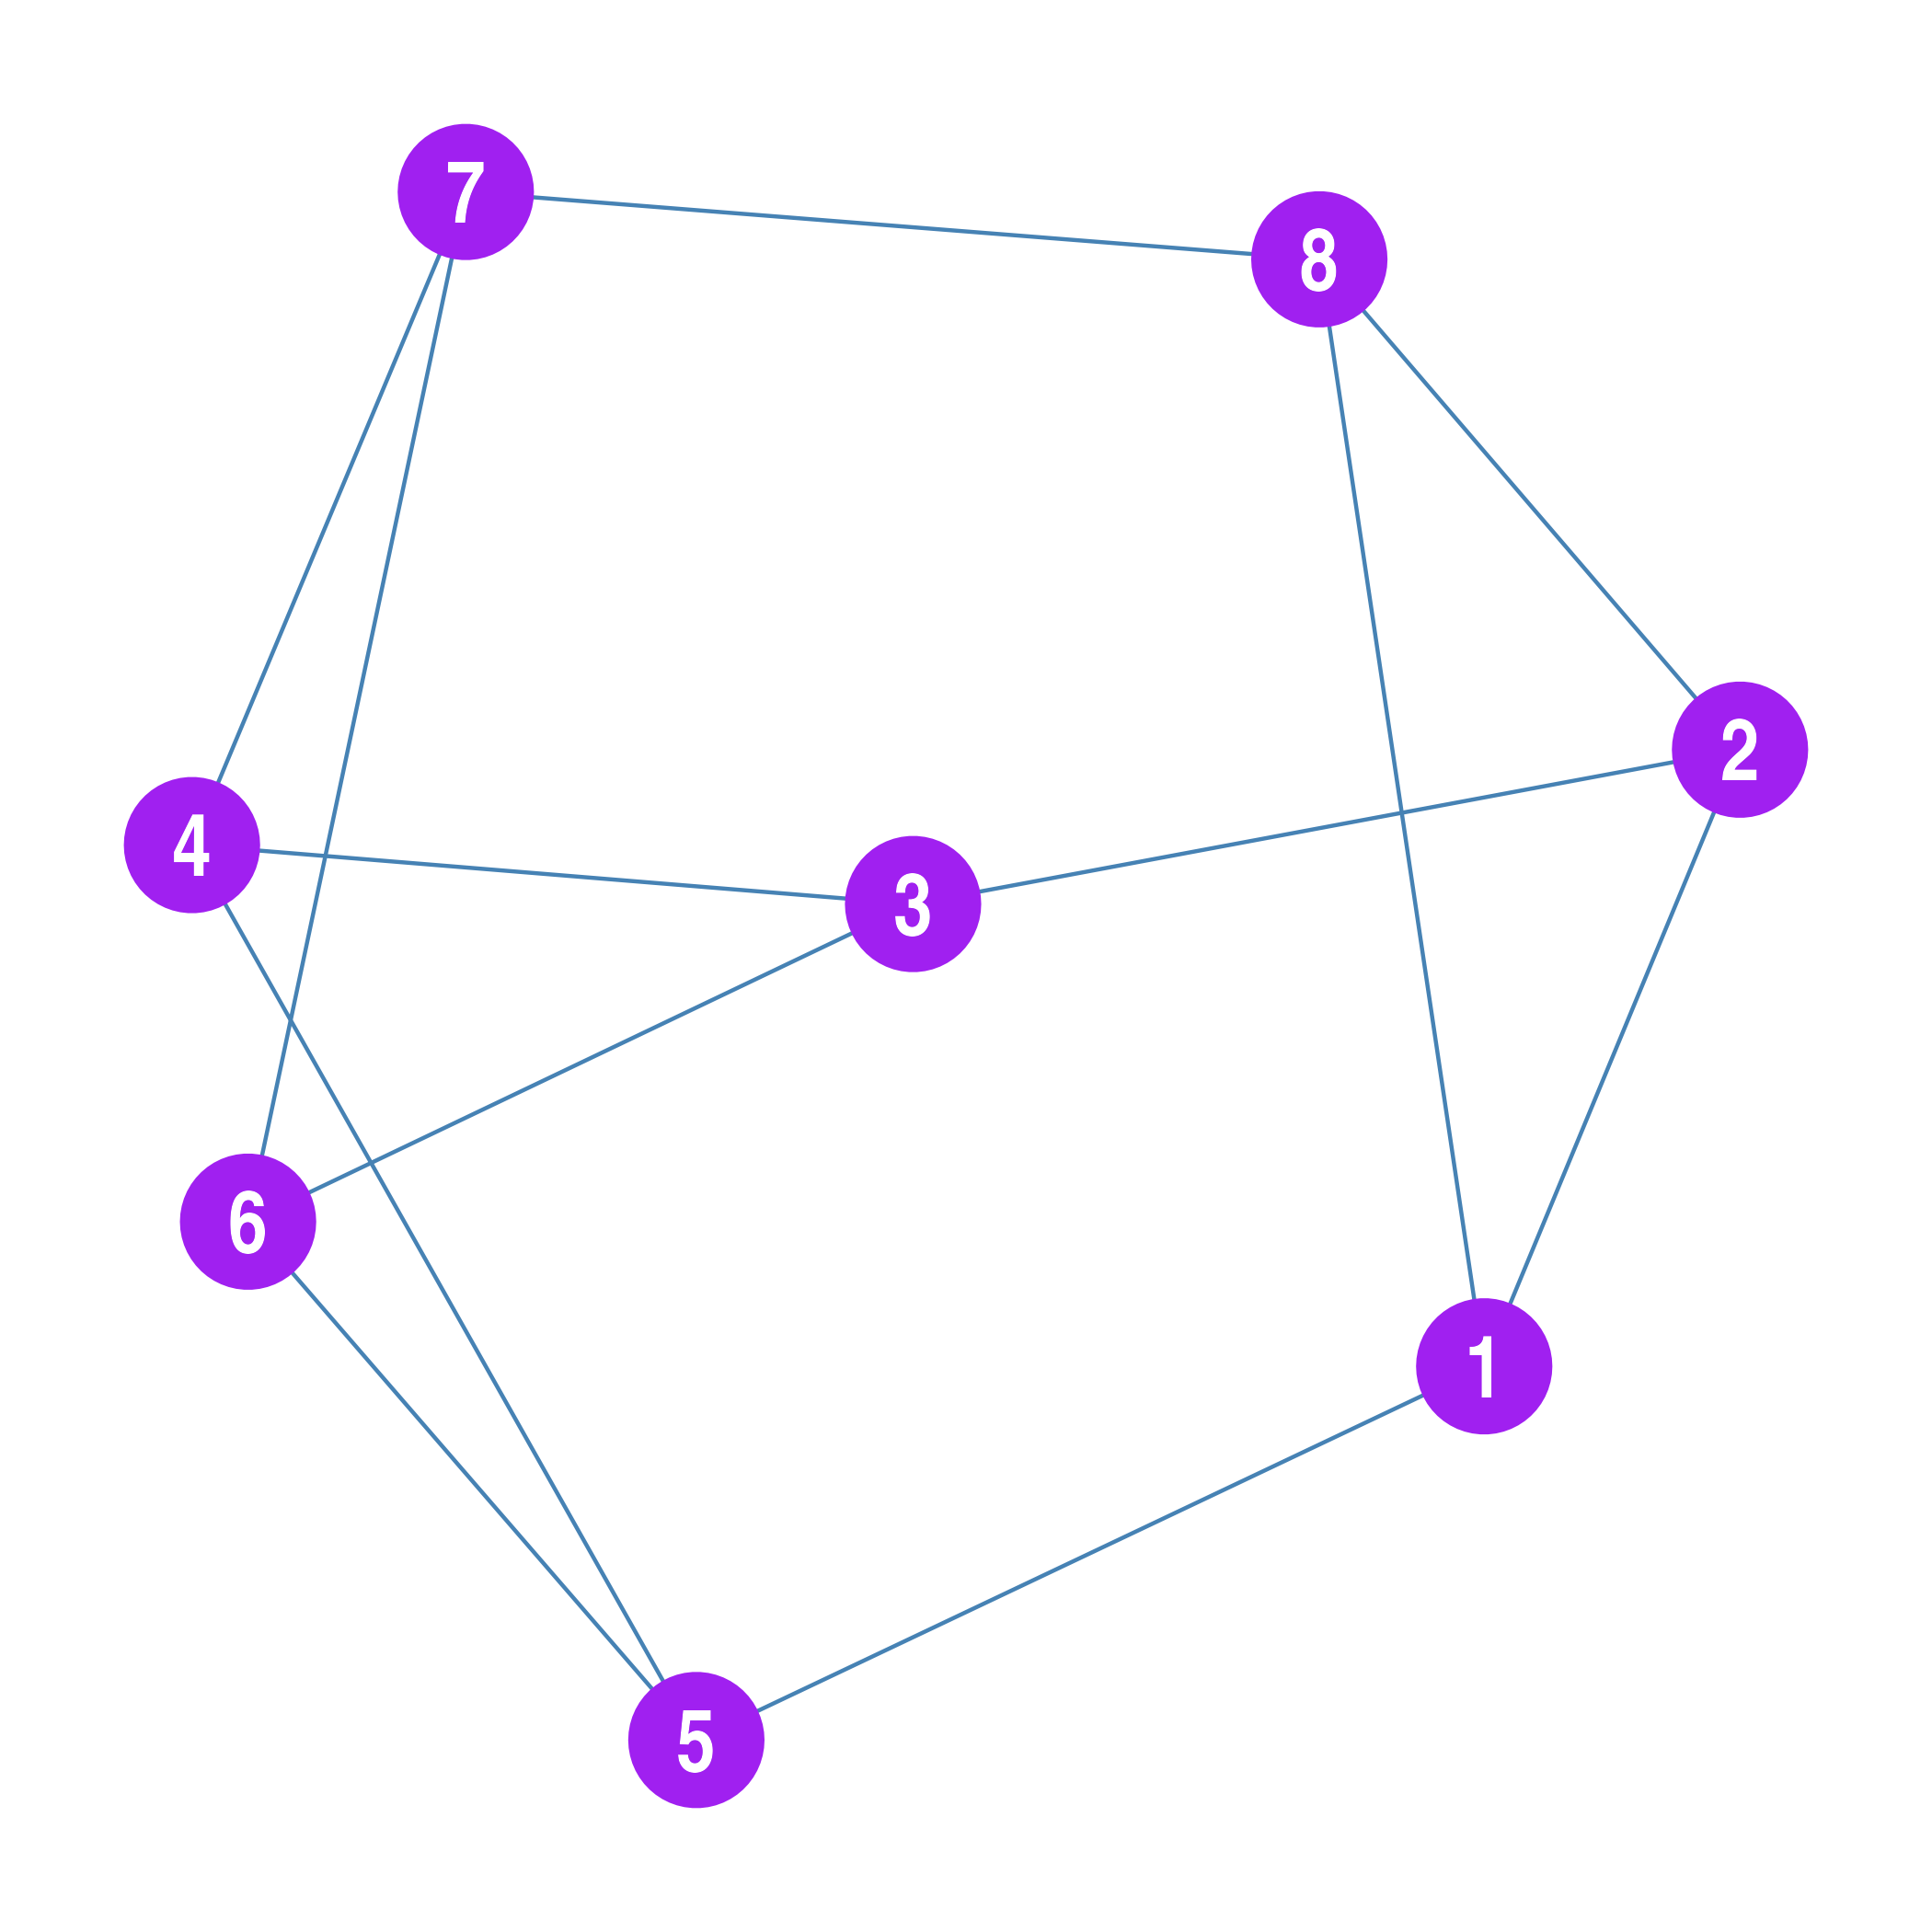
\includegraphics[width=\textwidth]{Plots/estrada-1a.png}
        \caption{Estrada Fig. 1(a) (Degree 3)}
        \label{fig:estrada1a}
    \end{subfigure}
    \hfill
    \begin{subfigure}[b]{0.45\textwidth}
        \centering
        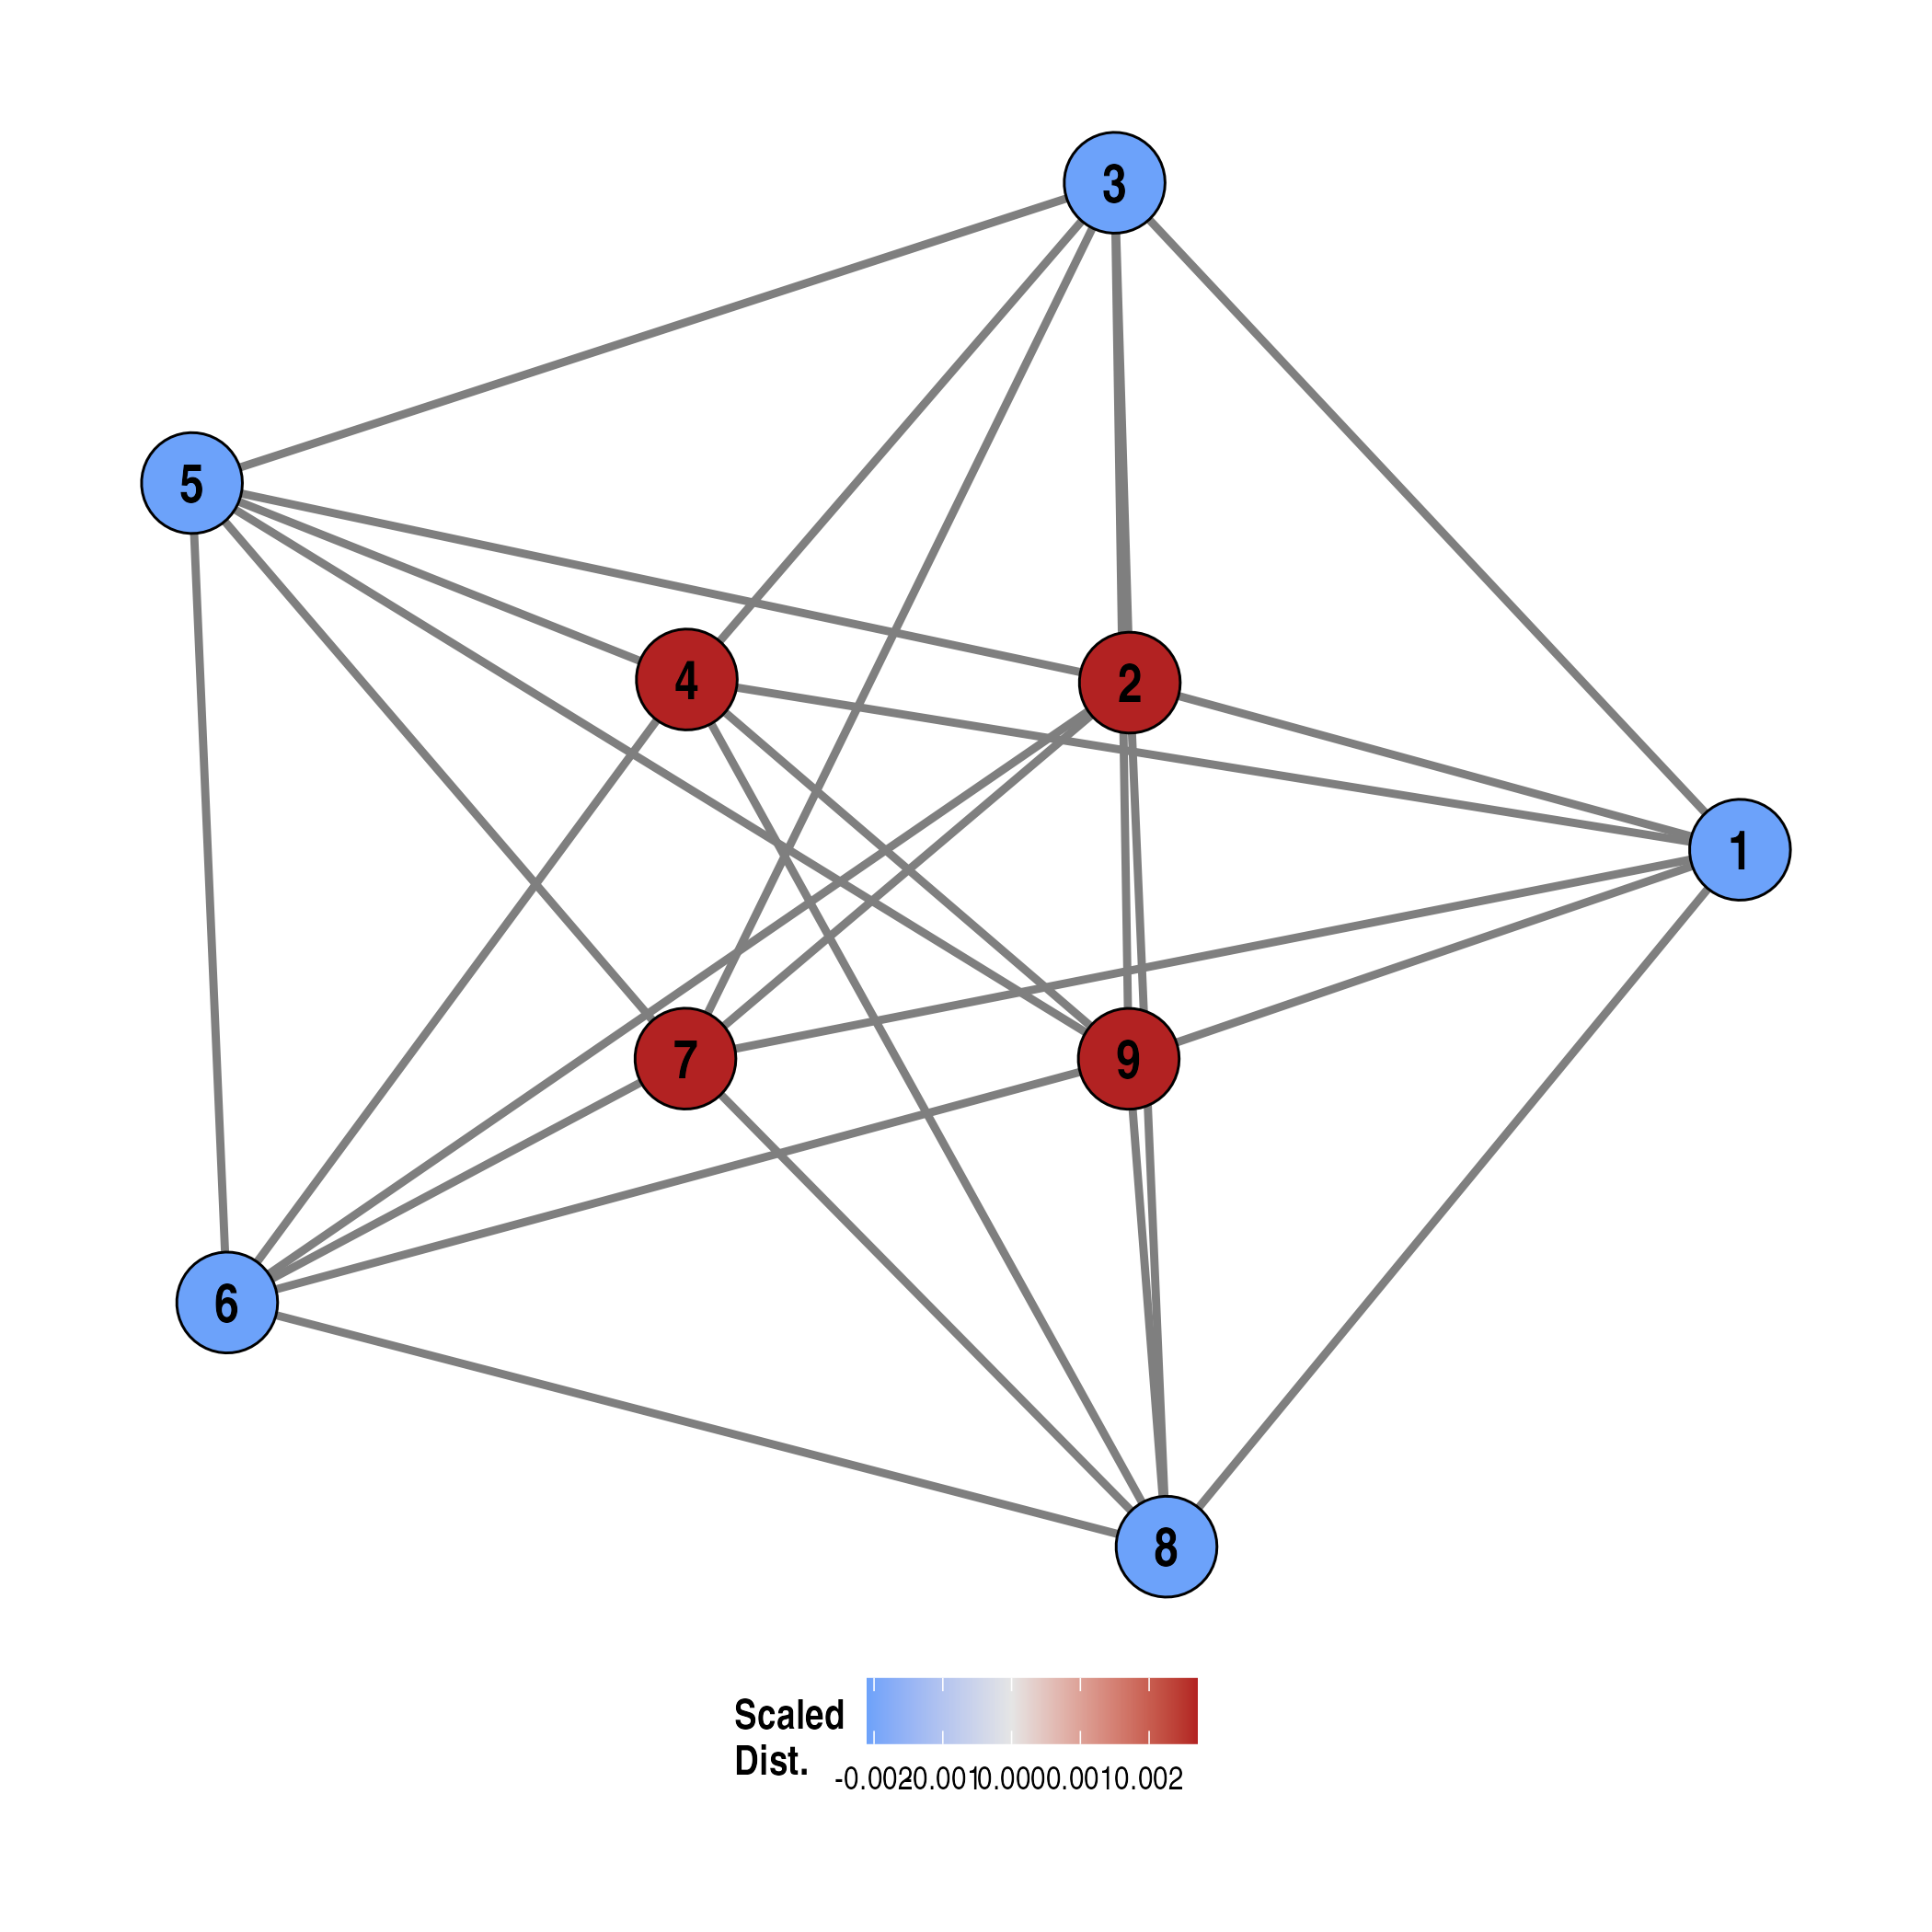
\includegraphics[width=\textwidth]{Plots/estrada-1b.png}
        \caption{Estrada Fig. 1(b) (Degree 6)}
        \label{fig:estrada1b}
    \end{subfigure}
    \caption{Distinction Centrality applied to the two regular graphs from \citet{estrada2005subgraph}. Nodes are perfectly differentiated according to their subgraph participation.}
    \label{fig:estrada}
\end{figure}

\begin{table}
\centering
\caption{\label{tab:estrada1a}Distinction centrality scores for the Estrada Fig 1(a) graph.}
\centering
\begin{tabular}[t]{lrrrr}
\toprule
Nodes & $\beta_i$ & $s_i$ & $\kappa_i$ & $\alpha$\\
\midrule
1, 2, 8 & 0.030 & 1 & 0.633 & 0.663\\
4, 6 & 0.008 & 1 & 0.655 & 0.663\\
3, 5, 7 & -0.036 & 1 & 0.699 & 0.663\\
\bottomrule
\end{tabular}
\end{table}

\begin{table}
\centering
\caption{\label{tab:estrada1b}Distinction centrality scores for the Estrada Fig 1(b) graph.}
\centering
\begin{tabular}[t]{lrrrr}
\toprule
Nodes & $\beta_i$ & $s_i$ & $\kappa_i$ & $\alpha$\\
\midrule
2, 4, 7, 9 & 0.003 & 1 & 0.849 & 0.852\\
1, 3, 5, 6, 8 & -0.002 & 1 & 0.854 & 0.852\\
\bottomrule
\end{tabular}
\end{table}


In the 8-node graph (Figure~\ref{fig:estrada1a}), nodes 1, 2, and 8 participate in triangles and receive the highest distinction score ($\beta_i = 0.030$). Nodes 4 and 6 participate in three squares and receive a moderate score ($\beta_i = 0.008$), while nodes 3, 5, and 7 participate in only two squares and receive the lowest score ($\beta_i = -0.036$). This matches the ranking of subgraph centrality perfectly. 

Similarly, in the dense 9-node graph (Figure~\ref{fig:estrada1b}), all nodes participate in the same number of triangles. The only structural difference is that nodes 2, 4, 7, and 9 participate in 45 squares, whereas the remaining nodes participate in 44. Distinction centrality is sufficiently sensitive to detect this minute topological variance, assigning a slightly higher score ($\beta_i = 0.003$) to the former group over the latter ($\beta_i = -0.002$).

The reason distinction centrality so gracefully detects structural motifs is due to its reliance on the node-deleted constraint metric ($\kappa_i$). Because constraint is calculated based on the spectral status of neighbors \emph{after} the focal node is removed, the presence of alternative local paths (such as the edges comprising triangles and squares) heavily dictates whether those neighbors retain their status. Thus, distinction centrality captures the same local network topology that Estrada explicitly sought to measure, doing so through the theoretical mechanism of structural redundancy and field constraint.
